% Template for Elsevier CRC journal article
% version 1.2 dated 09 May 2011

% This file (c) 2009-2011 Elsevier Ltd.  Modifications may be freely made,
% provided the edited file is saved under a different name

% This file contains modifications for Procedia Computer Science
% but may easily be adapted to other journals

% Changes since version 1.1
% - added "procedia" option compliant with ecrc.sty version 1.2a
%   (makes the layout approximately the same as the Word CRC template)
% - added example for generating copyright line in abstract

%-----------------------------------------------------------------------------------

%% This template uses the elsarticle.cls document class and the extension package ecrc.sty
%% For full documentation on usage of elsarticle.cls, consult the documentation "elsdoc.pdf"
%% Further resources available at http://www.elsevier.com/latex

%-----------------------------------------------------------------------------------

%%%%%%%%%%%%%%%%%%%%%%%%%%%%%%%%%%%%%%%%%%%%%%%%%%%%%%%%%%%%%%
%%%%%%%%%%%%%%%%%%%%%%%%%%%%%%%%%%%%%%%%%%%%%%%%%%%%%%%%%%%%%%
%%                                                          %%
%% Important note on usage                                  %%
%% -----------------------                                  %%
%% This file should normally be compiled with PDFLaTeX      %%
%% Using standard LaTeX should work but may produce clashes %%
%%                                                          %%
%%%%%%%%%%%%%%%%%%%%%%%%%%%%%%%%%%%%%%%%%%%%%%%%%%%%%%%%%%%%%%
%%%%%%%%%%%%%%%%%%%%%%%%%%%%%%%%%%%%%%%%%%%%%%%%%%%%%%%%%%%%%%

%% The '3p' and 'times' class options of elsarticle are used for Elsevier CRC
%% Add the 'procedia' option to approximate to the Word template
%\documentclass[3p,times,procedia]{elsarticle}
\documentclass[3p,times]{elsarticle}

%% The `ecrc' package must be called to make the CRC functionality available
\usepackage{ecrc}

%% The ecrc package defines commands needed for running heads and logos.
%% For running heads, you can set the journal name, the volume, the starting page and the authors

%% set the volume if you know. Otherwise `00'
\volume{00}

%% set the starting page if not 1
\firstpage{1}

%% Give the name of the journal
\journalname{Future Generation Computing Systems}

%% Give the author list to appear in the running head
%% Example \runauth{C.V. Radhakrishnan et al.}
\runauth{L. Miroslaw et al.}

%% The choice of journal logo is determined by the \jid and \jnltitlelogo commands.
%% A user-supplied logo with the name <\jid>logo.pdf will be inserted if present.
%% e.g. if \jid{yspmi} the system will look for a file yspmilogo.pdf
%% Otherwise the content of \jnltitlelogo will be set between horizontal lines as a default logo

%% Give the abbreviation of the Journal.  Contact the journal editorial office if in any doubt
\jid{fgcs}

%% Give a short journal name for the dummy logo (if needed)
\jnltitlelogo{FGCS}

%% Provide the copyright line to appear in the abstract
%% Usage:
%   \CopyrightLine[<text-before-year>]{<year>}{<restt-of-the-copyright-text>}
%   \CopyrightLine[Crown copyright]{2011}{Published by Elsevier Ltd.}
%   \CopyrightLine{2011}{Elsevier Ltd. All rights reserved}
\CopyrightLine{2011}{Published by Elsevier Ltd.}

%% Hereafter the template follows `elsarticle'.
%% For more details see the existing template files elsarticle-template-harv.tex and elsarticle-template-num.tex.

%% Elsevier CRC generally uses a numbered reference style
%% For this, the conventions of elsarticle-template-num.tex should be followed (included below)
%% If using BibTeX, use the style file elsarticle-num.bst

%% End of ecrc-specific commands
%%%%%%%%%%%%%%%%%%%%%%%%%%%%%%%%%%%%%%%%%%%%%%%%%%%%%%%%%%%%%%%%%%%%%%%%%%

%% The amssymb package provides various useful mathematical symbols
\usepackage{amssymb}
\usepackage{url}
%% The amsthm package provides extended theorem environments
%% \usepackage{amsthm}

%% The lineno packages adds line numbers. Start line numbering with
%% \begin{linenumbers}, end it with \end{linenumbers}. Or switch it on
%% for the whole article with \linenumbers after \end{frontmatter}.
%\usepackage{lineno}

%% natbib.sty is loaded by default. However, natbib options can be
%% provided with \biboptions{...} command. Following options are
%% valid:

%%   round  -  round parentheses are used (default)
%%   square -  square brackets are used   [option]
%%   curly  -  curly braces are used      {option}
%%   angle  -  angle brackets are used    <option>
%%   semicolon  -  multiple citations separated by semi-colon
%%   colon  - same as semicolon, an earlier confusion
%%   comma  -  separated by comma
%%   numbers-  selects numerical citations
%%   super  -  numerical citations as superscripts
%%   sort   -  sorts multiple citations according to order in ref. list
%%   sort&compress   -  like sort, but also compresses numerical citations
%%   compress - compresses without sorting
%%
%% \biboptions{comma,round}

% \biboptions{}

% if you have landscape tables
\usepackage[figuresright]{rotating}

% put your own definitions here:
%   \newcommand{\cZ}{\cal{Z}}
%   \newtheorem{def}{Definition}[section]
%   ...

% add words to TeX's hyphenation exception list
%\hyphenation{author another created financial paper re-commend-ed Post-Script}

% declarations for front matter

\usepackage[utf8]{inputenc} % set input encoding (not needed with XeLaTeX)
\usepackage{wrapfig} 
\usepackage{subcaption}
\usepackage{graphicx} % support the \includegraphics command and options

%%% PACKAGES
%\usepackage{booktabs} % for much better looking tables
%\usepackage{tikz}
\usepackage{todonotes}
%\usepackage{array} % for better arrays (eg matrices) in maths
%\usepackage{paralist} % very flexible & customisable lists (eg. enumerate/itemize, etc.)
%\usepackage{verbatim} % adds environment for commenting out blocks of text & for better verbatim
%\usepackage{subfig} % fmake it possible to include more than one captioned figure/table in a single float
% These packages are all incorporated in the memoir class to one degree or another...

%%% SECTION TITLE APPEARANCE
%\usepackage{sectsty}
%\allsectionsfont{\sffamily\mdseries\upshape} % (See the fntguide.pdf for font help)
% (This matches ConTeXt defaults)

%%% ToC (table of contents) APPEARANCE
%\usepackage[nottoc,notlof,notlot]{tocbibind} % Put the bibliography in the ToC
%\usepackage[titles,subfigure]{tocloft} % Alter the style of the Table of Contents
%\renewcommand{\cftsecfont}{\rmfamily\mdseries\upshape}
%\renewcommand{\cftsecpagefont}{\rmfamily\mdseries\upshape} % No bold!

%%% END Article customizations

\DeclareGraphicsExtensions{.pdf,.png,.jpg}
\graphicspath{ {../figs/} }

\begin{document}

\begin{frontmatter}

%% Title, authors and addresses

%% use the tnoteref command within \title for footnotes;
%% use the tnotetext command for the associated footnote;
%% use the fnref command within \author or \address for footnotes;
%% use the fntext command for the associated footnote;
%% use the corref command within \author for corresponding author footnotes;
%% use the cortext command for the associated footnote;
%% use the ead command for the email address,
%% and the form \ead[url] for the home page:
%%
%% \title{Title\tnoteref{label1}}
%% \tnotetext[label1]{}
%% \author{Name\corref{cor1}\fnref{label2}}
%% \ead{email address}
%% \ead[url]{home page}
%% \fntext[label2]{}
%% \cortext[cor1]{}
%% \address{Address\fnref{label3}}
%% \fntext[label3]{}

\dochead{Big Data in the Cloud}
%% Use \dochead if there is an article header, e.g. \dochead{Short communication}
%% \dochead can also be used to include a conference title, if directed by the editors
%% e.g. \dochead{17th International Conference on Dynamical Processes in Excited States of Solids}

\title{Unified cloud orchestration framework for elastic high performance computing in the cloud}
% NAFEMS: A unified framework for orchestration of numerical simulations in the Windows Azure cloud platform

%% use optional labels to link authors explicitly to addresses:
%% \author[label1,label2]{<author name>}
%% \address[label1]{<address>}
%% \address[label2]{<address>}

\author[hsr]{Lukasz Miroslaw}
\author[hsr]{Vladimir Baros}
\author[hsr]{Michael Pantic}
\author[hsr]{Henrik Nordborg}

\address[hsr]{Institute for Energy Technology, Hochschule Rapperswil, Switzerland}
\address[eth]{ETH Zurich, Switzerland}

\begin{abstract}
%The efficient use of numerical simulations, such as computational fluid dynamics, requires significant computing power, usually only available through large and expensive cluster systems. This effectively hinders small and medium organizations from simulating, as those clusters need to be sized sufficiently large and highly utilized to be profitable.
%Those problems can be solved using elastic, pay-per-use cloud computing. In this paper, we show how well different problems scale with different machines and cluster configurations within Microsoft Azure. We also focused on decreasing computational time without increasing the total costs of operation, using dynamic, short-term allocation of nodes. Additionally, we give a short introduction on how MPI jobs can be executed with no pre-existing infrastructure. Performance estimates and comparisons with traditional on-site clusters are made using the HPL and HPCG benchmarks.
%\todo[inline]{maybe say something about the goal of lowering the entry barriers for simulating.} 

Numerical simulations stand in need for scalable computing power, storage and high availability that can be provided only through expensive and large clusters. While this is a preferred option for research institutions, government agencies and large companies, small and medium enterprises can often not afford large investments. Apparently, the reasonable return of investment is only possible when the clusters are highly utilized and sized optimally depending on the actual demands. 
Those problems can be solved using elastic, pay-per-use cloud computing platforms. Still, accessing own applications in the cloud is a tedious task and requires a significant amount of effort and expertise in cloud computing. Bringing a specific application to the IaaS infrastructure is difficult to achieve. A numerical application that needs to be deployed is usually a command line-tool that requires a similarly complex deployment steps as on the private cluster, e.g. installation, configuration as well as setting up system specific services and network policies. This can be too cumbersome for a domain engineer or a scientist. A simple mechanism is needed to simplify the whole process and lower the entry barrier for cloud-based simulations.
Therefore, we present a unified framework to submit an application directly to the cloud in a simple way. The platform integrates Microsoft Azure specific HPC libraries with PowerShell commandlets to ease the submission process while keeping the desired command line environment. The framework provides tools with the ability to deploy necessary number of virtual machines dynamically, submit the packed application together with input and configuration files, execute the simulation and, once the results are ready, download them to the local machine and stop the virtual machines. 
We demonstrate our framework in orchestration of three use cases: deployment of PETSc numerical simulation tool and HPCG benchmark suite and ANSYS. In addition, we also show how well different computational problems scale with different machines and cluster configurations within Microsoft Azure. We also discuss the costs of simulations in different configuration scenarios as well as provide performance estimates and comparisons with traditional on-site clusters.


\end{abstract}

\begin{keyword}
microsoft azure \sep high performance computing
%% keywords here, in the form: keyword \sep keyword

%% PACS codes here, in the form: \PACS code \sep code

%% MSC codes here, in the form: \MSC code \sep code
%% or \MSC[2008] code \sep code (2000 is the default)

\end{keyword}

\end{frontmatter}

%\linenumbers 

\section{Introduction} 
\label{sec:introduction}
% why we need a cloud

Computational fluid dynamics (CFD) and numerical simulations are powerful methods to support engineering designs and reduce development costs in both industry and research. Since Navier-Stokes equations have been formulated in XIX century, it was possible to study the motion of viscous fluids and  model many physical phenomena of a great importance for industry, science and society. For example CFD can be used to model the water flow in the pipe, the development of the electrical arc, blood flow in the human aorta, ocean currents or an air flow around a wing. 

The recent advances in information technology made it possible to analyze larger models with higher precision in shorter time. This requirement calls for large amount of computational power, which typically is provided by large, expensive on-premise clusters. As such systems are unavailable to small or medium enterprises (SMEs) that have limited access to clusters, the numerical simulations are often not considered as viable alternatives to traditional prototyping. On the other hand, the research groups are not capable to solve their models locally, making them dependent on the external cluster.

%\todo[inline]{describe existing tools} 

% what is the cloud, what are the problems
Cloud computing has become ubiquitous due to its flexibility and cost-efficiency. It has clear advantages over traditional on-premise systems for SMEs with limited budgets as no direct investment is needed and machines can be rented on an hourly basis. Users benefit from the cloud through a possibility to launch jobs of different size and scalability and the cloud operators achieve economies of scale by building large data centers where the resources can be shared between different workloads. \\
An increasing amount of computing power is now hosted on cloud platforms such as Amazon Elasting Compute (EC2) \cite{ec2}, Cloud Foundry Google Compute Engine \cite{google} or Microsoft Azure \cite{azure} and more and more software and services is being hosted in the cloud. Many independent software vendors (ISV) started to offer cloud services to scale scientific applications for specific industries. For example many ISVs like Ciespace, Ubercloud, Sabalcore, Univa, Penguin Computing provide cloud services for weather research, computational fluid dynamics, structural mechanics, quantitative finance, combustion, electromagnetics and molecular dynamics \cite{theuebercloud}. They offer access to VMs with a preinstalled software or a web portal where the scientific applications, such as ANSYS, Gromacs, OpenFOAM or Gerris solver can be executed \cite{Popinet2003}.

%of using the cloud is the security. The jobs are executed on a hardware in unknown location that is not fully controlled by the user. The cloud providers do their best to convince the user that the data is saved by using different security policies. 
While this may be a satisfying solution for some of the users, ability to run own or a third-party software on the cloud infrastructure requires much more complicated procedure. A scientific application that needs to be deployed is usually a command line-tool that requires a similarly complex deployment steps as on the private cluster such as installation, configuration as well as setting up system specific services and network policies. Access to the deployed applications from the local machine is also a tedious procedure and requires a significant amount of effort. This is why this scenario is often too cumbersome for a domain engineer or a scientist.  

A simple mechanism is needed to simplify the whole process and lower the entry barrier for cloud-based numerical simulations. Such mechanisms exist for Amazon EC2 \cite{ec2} \cite{eucalyptus} but Microsoft Azure still lacks an easy-to-use framework to simplify cloud  orchestration, although it is a platform that is well positioned on the market \cite{Garg2013}.

We present a unified framework we called SimplyHPC to submit a distributed application directly to Microsft Azure in a simple way. The platform integrates Azure specific HPC libraries with PowerShell commandlets to ease the submission process while keeping the desired command line environment. The framework provides tools with the ability to deploy necessary number of virtual machines dynamically, submit the packed application together with input and configuration files, execute it as a cloud service using Message Passing Interface (MPI) and, once the results are ready, download them to the local machine and stop the virtual machines. 

Our paper focuses on following aspects. Chapter \ref{sec:architecture} describes the main components of the proposed framework as well the platform architecture. Chapter \ref{sec:results} demonstrates the utility of the tool on two scientific applications, chapter \ref{sec:costs} examines the economical aspects of running in the cloud. The paper ends with conclusions and future plans.

%\todo[inline]{Wie auf das 100h/20chf oder 1h fuer 2000chf problem eingehen unten ?}

%VERY INTERESTING

%	\item[II] We measured how well different applications scale on a cloud computing platform (Microsoft Azure), evaluating feasibility and %cost of operation for different applications and optimizing the machine count / machine size ratio to get as much GFLOPs per \$ as possible.

%\end{itemize}

\section{Background}

\subsection{Motivation}

% there are a few frameworks, not for Azure
Each of the previously mentioned cloud platforms offers different strategies to communicate with the cloud infrastructure and different virtualization procedures. The user is free to manage the cloud resources by using standard approach, or use cloud orchestrators that automate the management of the cloud-based infrastructure. 

\begin{description}
\item[Complex deployment] The IaaS cloud requires the user to deploy the application in a similar and often complex way as on the local cluster. Cloud orchestrators manage the interactions and interconnections among cloud-based and on-premises business units as well as expose various automated processes and associated resources. They have become a desired alternative to standard deployment procedures because of lower level of expertise and reduced deployment time. Tools for cloud orchestration and vertical and horizontal scaling are fundamental to the adoption of the framework aiming at simplifying the whole procedure.

\item[Complicated access] Although cloud orchestrators play an important role, still there are only a few easy to use, out-of-the box platforms that simplify deployment, monitoring and accessing scientific applications in the cloud. Companies offering cloud-based software in PaaS model limit their offering to applications of the highest commercial impact while neglecting other types of software such as numerical simulations \cite{CloudStack} \cite{OpenStack}. The best situation is in Amazon EC2 where frameworks to simplify the process of orchestration of specific scientific applications exist. Wong and Goscinski propose a unified framework composed of a series of scripts for running gene sequencing analysis jobs through a web portal \cite{Wong2013} on Amazon EC2 (IaaS) infrastructure. For this purpose they designed a HPC service software library for accessing high level HPC resources from the IaaS cloud and demostrate their framework in running mpiBLAS \cite{mpiBlas}. Balgacem et al. measured the multiphase flow on a hybrid platform combined with Amazon $EC2$ and a private cluster \cite{BenBelgacem2015}. Morpho is a modified version of Hadoop MapReduce framework that decouples storage and computation into physical and virtual clust ers to reduce costly data movement of user data \cite{Lu2014}. The authors demonstrate the efficiency of the  framework in text mining application compared with the Hadoop MapReduce running in Amazon mode. Twister4Azure is a MapReduce frameworks designed specifically for Microsoft Azure. It extends the native Hadoop framework in Azure cloud platform and provides multi-level data caching mechanism to overcome the latencies of cloud services as well as a decentralized task scheduling to avoid single point of failure. Still, the framework requires a programming knowledge since it is relased as .NET Project. The platform has been demonstrated in applications that are well fitted to MapReduce paradigm, such as BLAS sequence searching or KMean Clustering. Marozzo et. al \cite{catlett2013cloud} present a web-based framework for running pre-defined workflows composed of web services in Microsoft Azure. The authors demonstrate the framework in data mining applications by deploying an execution workflow running a single classification algorithm and measure strong scalability in classifying different data sets that were previously partitioned. Unfortunately, it is not clear if the algorithm was multi- or single-threaded or if is possible to add own applications to the framework that are no exposed as web-services and not related to data mining. 
Another interesting frameworks are Eucalyptus \cite{eucalyptus} or CloudStack \cite{CloudStack} that were designed to deploy IaaS hybrid clouds, e.g. scalable IaaS cloud computing platform composed of a private cloud and public one based on Amazon EC2.

\end{description}


%many scientific groups run their scientific code on the cloud
%Since that time many groups attempted to evaluate scientific code on cloud platforms. 

%Windows Azure, a platform offered by Microsoft is a well established platform for high performance computing that 
%\todo[inline]{List more examples} 


%In this paper we focus on th
%Frameworks to simplify the process of orchestration of the scientific applications have also been developed. Wong and Goscinski propose a unified framework that integrates an HPC service library, Amazon EC2 for running mpiBLAST jobs through a web portal \cite{Wong2013}. 
% Their framework exposes 

%TODO: Add more frameworks. 

%Still, there are only a few frameworks that simplify deployment on Windows Azure. 

\subsection{Microsoft Azure}

Microsoft Azure is a cloud computing platform providing three types of VM roles. Web and Worker roles in PaaS model provide a set of predefined cloud services for web applications and scalable applications, respectively. VM roles in IaaS model are just bare machines deployed with a specific OS. The platform is well positioned on the market and is competitive to other cloud providers \cite{cloudScores} \cite{twister4azure} with a large user base and third-party cloud services. As of 2015, ten types of different instances available (see \ref{tab:azureVMs}). Computational costs on Microsoft Azure depend on the number of cores, the type of machine and the time of effective usage. The time of effective usage is the time between set-up of the virtual machine and its tear-down, regardless of the actual usage or workload. \\
A8 and A9 are special Azure VM instances which include Infiniband network stack with low latency and Remote Direct Memory Access (RDMA) enabled. Unfortunately, the specification of the CPUs is provided only for these instances, for other VMs only the number of cores, RAM and disk size is provided. 
 
%TODO: extend the list

	\begin{center}
	\begin{table}
				\begin{tabular}{|c|c|c|c|c|c|}
			\hline
			Instance & Cores & RAM     & Disk size & CPU & Price                    \\ \hline
				A0     & 1     & 0.75 GB & 20 GB      & - & \$0.02/hr (\~\$15/mo)    \\ \hline
				A1     & 1     & 1.75 GB & 70 GB      & - & \$0.09/hr (\~\$59/mo)    \\ \hline
				A2     & 2     & 3.5 GB  & 135 GB     & - & \$0.18/hr (\~\$116/mo)   \\ \hline
				A3     & 4     & 7 GB    & 285 GB     & - & \$0.36/hr (\~\$232/mo)   \\ \hline
				A4     & 8     & 14 GB   & 605 GB     & - & \$0.72/hr (\~\$463/mo)   \\ \hline
				A5     & 2     & 14 GB   & 135 GB     & - & \$0.33/hr (\~\$253/mo)   \\ \hline
				A6     & 4     & 28 GB   & 285 GB     & - & \$0.66/hr (\~\$513/mo)   \\ \hline
				A7     & 8     & 56 GB   & 605 GB     & - & \$1.32/hr (\~\$1019/mo)  \\ \hline
				A8     & 8     & 56 GB    & 382 GB    & Intel Xeon E5-2670 & \$2.45/hr (\~\$1,771/mo) \\ \hline
				A9     & 16    & 112 GB  & 382 GB     & Intel Xeon E5-2670 & \$4.90/hr (\~\$3,541/mo) \\ \hline
			\end{tabular}
			\label{tab:azureVMs}
			\caption{Microsoft Azure VM instances. Price list retrieved in December 2014.}
	\end{table}
\end{center}
 

Cloud computing platform can be used either as Infrastructure as a Service (IaaS) or Platform as a Service (PaaS), each offering different level of control and complexity. IaaS model exposes Virtual Machines with no additional software or services installed, except a predefined operating system (OS). The user is responsible for system maintenance and software installations. Virtual Machines are usually accessed by SSH protocol or Remote Desktop Controller, depending on the selected OS. PaaS architecture is exposed as light-weight virtual machines, called {\it Cloud Services}. They are much simpler to use: instead of configuring the Virtual machines the user uploads a packaged application together with the configuration files. This ''deployment package'' is then installed on a fresh virtual machine automatically and exposes its features to the user in seamless way. If there are any configuration changes the cloud service is removed and reinstalled on the virtual machine together with the updated deployment package. Such a procedure takes usually a few minutes and is  attractive in terms of rental costs of the cloud because the created VM is immediately deleted after usage. \\
Microsoft Azure provides both types of services for different types of applications. IaaS are provided for non-standard, user-defined applications while PaaS offer easy access to mostly used services such as web servers, applications server or message brokers. Separate entities provide infrastructure for highly available and scalable data storage. Microsoft Azure exposes four storage types to store, manage and control data in the cloud: Blob, Table, Queue and File. Each storage type is able to host different types of data of arbitrary sizes, namely binary files of any type, structured datasets, messages and shared files, respectively. We decided to take advantage of the cloud service (PaaS) to simplify the orchestration procedure and use Blob and Table storage entities for data management. 

\subsection{HPC Pack}

HPC Pack is a framework developed by Microsoft for monitoring, executing and running jobs in both premise and on Azure platform. It contains a set of deployment, monitoring, administration and job scheduling tools for running HPC applications. Originally it was created for Windows HPC clusters composed of dedicated on-premise compute nodes and workstation computers and the support for Microsoft Azure has been added on top of that. HPC Pack exposes functionality that is typical for cluster management software such as deployment of clusters with different configurations, scheduler that maximizes an utilization of the cluster based on priorities, policies and usage patterns and a batch system for submission of multiple short and long running jobs with different amount of resources. The framework also allows for deployment of hybrid clouds, for example to deploy a head node on-premise and control Azure PaaS nodes or to deploy the head node as a IaaS VM and control PaaS VMs from the local machine. It is a recommended framework to control the Azure cloud.

\subsection{Numerical Software}
\label{sec:numerical}

Sparse linear algebra inspired the use cases presented in this study. Large sparse matrices are generated during the disretization of partial differential equations and often appear in scientific or engineering applications. We have selected two scientific software tools, namely PETSc and High Performance Conjugate Gradient (HPCG) Benchmark to demonstrate the utility of our framework, to measure the performance on both Microsoft Azure and local cluster. 
The High Performance Conjugate Gradient \(HPCG\) Benchmark \cite{Heroux2013} is a benchmark program that solves a sparse linear system during discretization of a three-dimensional heat diffusion problem on a semi-regular grid. Domain decomposition with an additive Schwarz preconditioned conjugate gradient method is used to solve the problem where each subdomain is preconditioned using a symmetric Gauss-Seidel sweep. This benchmark is much more relevant than the LINPACK benchmark that is currently used by $Top500$ which is a solver of a dense system of linear equations. As such LINPACK favors computers with very high floating-point computations an streaming memory systems. Colaesed access to memory is easier to achieve when matrix-matrix multiplications and similar operations are performed on dense matrices. While this is a case for many scientific problems, the LINPACK does not adequately expressed the performance of applications that are based on different memory access patterns, in particular the ones stemming from finite volume of finite element methods. HPCG, as more representative, has been used to benchmark the largest clusters such as Tianhe-2 \cite{Xianyi2014} has started to become more popular in definition of Top500 list. It provides a simple way to measure the performance on easy-to-scale case in MFLOPS across multi-node mode. \\
PETSc is a library with a set of nonlinear and Krylov-subspaces linear solvers with the possibility to run external direct solvers as well as GPU-based kernels. Krylov space methods are considered to be as one of ten most important classes of numerical methods and large sparse matrix eigenvalue problems are present in most scientific computing applications \cite{Gutknecht2005}. This is one the reasons why this software is wide used in multiple scientific disciplines such as acoustics, aerodynamics, computational fluid dynamics, combustion and ocean dynamics just to name a few \cite{petsc-efficient}.\\
In addition to the numerical tools, we have selected ANSYS CFX, a high performance fluid dynamic software that is well recognized in industry and has been successfully applied to different fluid flow problems. It simulates many fluid phenomena including steady-state, transient flows of both laminar and turbulent nature as well as multiphase flows, heat transfer and radiation. Since the installation folder must be accessible by all compute nodes, we additionally created a storage file service which provides the installation files to the compute nodes. During the deployment of the compute nodes, the ANSYS CFX installation folder is being mounted on all machines, using the same drive letter. Once ANSYS CFX is accessible by all compute nodes, other preparation steps such as the installation of MPI and SPMD can be scripted with our framework. We will show the corresponding performance studies in Chapter \ref{sec:results}.

\section{SimplyHPC Architecture}
\label{sec:architecture}

%Blob storage is used to upload deployment templates, upload job data and download results. 
%Table storage is used to indicate to our Cloud Service that the job is waiting to be executed and that there is a result to be downloaded.

SimplyHPC framework enables users without any cloud-related knowledge to run their single- and multi-threaded applications on the cloud instead of a local machine or a private cluster. This way they can take advantage of the computing power of Microsoft Azure cloud and release their local resources for other tasks. The software hides from the user the whole cloud-related complexity, i.e. required installation and deployment procedures are not exposed to the user and performed in the background. Similarly, all necessary Microsoft Azure and third-party dependencies are included and configured automatically. \\
The whole process of exposing the scientific application in the cloud can be controlled with the command line scripts called commandlets. 

\begin{table}
	\centering		
		\begin{tabular}{|l|l|}
		\hline
      \textbf{Commandlet} & \textbf{Description} \\ \hline
      NewAzureService & Create a new cloud service and the cluster \\ \hline
			NewAzureJob & Create and execute a new job \\ \hline
			NewAzureParameters & Create a set of parameters required by other commandlets    \\ \hline
			GetJobStatus & Get the status of a given job    \\ \hline
			GetJobResults & Get the results of a given job  \\ \hline
			GetAvailableRoleSizes & Get Available VMs with their roles and sizes \\ \hline
			RemoveAzureJobs & Remove Azure Jobs such as unfinished jobs \\ \hline
			RemoveAzureService & Remove the cloud service and destroy the cluster \\ \hline
    \end{tabular}
	\caption{Commandlets of SimplyHPC framework.}
	\label{tab:CommandletsOfSimplyHPC}
\end{table}

The commandlets are PowerShell modules executed in a specific order and realize specific tasks needed to deploy a scientific application in the cloud, execute it, download the results back to the user and destroy the cluster (see Tab~\ref{tab:CommandletsOfSimplyHPC}). The commandlets call methods from Controller API and prepare the application to be deployed as a cloud service. 
%The module defines how many instances are run and other settings Template mechanism is  and Job Scheduler. 
The Controller is a shared library with the high-level API that takes advantage of Microsoft Azure Cloud API to assign computational jobs to Azure resources, to communicate with deployment entities and Microsoft Azure components such as Storage. Commandlets use this API to automatize the set-up and deployment tasks as well as uploading the job and downloading the results. 
% In the full paper : high-availability subsection. Blob and Table storage is used to ensure the data mirroring and high-availability provided by the cloud
The configuration of the cloud service is managed by the Deployment Template Module (DTM). DTM is a library with a set of C\# interfaces for running MPI jobs in the cloud service. Once uploaded the cloud service is invoked as a windows service on each node of the cluster where it installs Microsoft MPI library and the deployed application automatically.
In addition, the service periodically checks the blob and table storage for new enqueued jobs. Every new job is automatically executed,  removed from the queue and the new results are downloaded to the local machine. This way the service takes also the responsibility of a simple job scheduler that executed the jobs one by one on available resources. \\
The architecture of the whole system is presented in Fig. \ref{fig:architecture} while the deployment procedure is presented in Section \ref{sec:deploymentProcedure}. 

\subsection{High Availability}
\label{sec:high_avilability}
Each of the deployed instance has access to a local drive. Although theoretically it is possible to store the job data in this location, such a mechanism is not fail-safe. A failure of any of the nodes will endanger the whole execution since part of the results will be missing.\\
A simple mechanism was implemented to ensure the data persistence and high availability. For that purpose a special components of Microsoft Azure were used, called Azure Storage. Azure storage is a massively scalable, durable and highly available auto-partitioning system that automatically load-balance data based on traffic. It scales automatically when the application demands more resources in terms of amount of data and the number of requests. It is accessible from either from the deployed nodes or the on-premise machine. SimplyHPC uses Blob and Table storage to separate the data from other system components. The packed application, job data, its input and output results are stored in the Blob storage while Table Storage is used to store the job metadata and information about it status. Both the Table and Blob Storage entities are accessible to local and remote machines. Every time the job is uploaded a new entry with the job metadata is appended to the Table. %Job Scheduler configured as a windows service on the head node examines the Table regularly and executes the jobs one by one. \\

\begin{figure}
\centering
  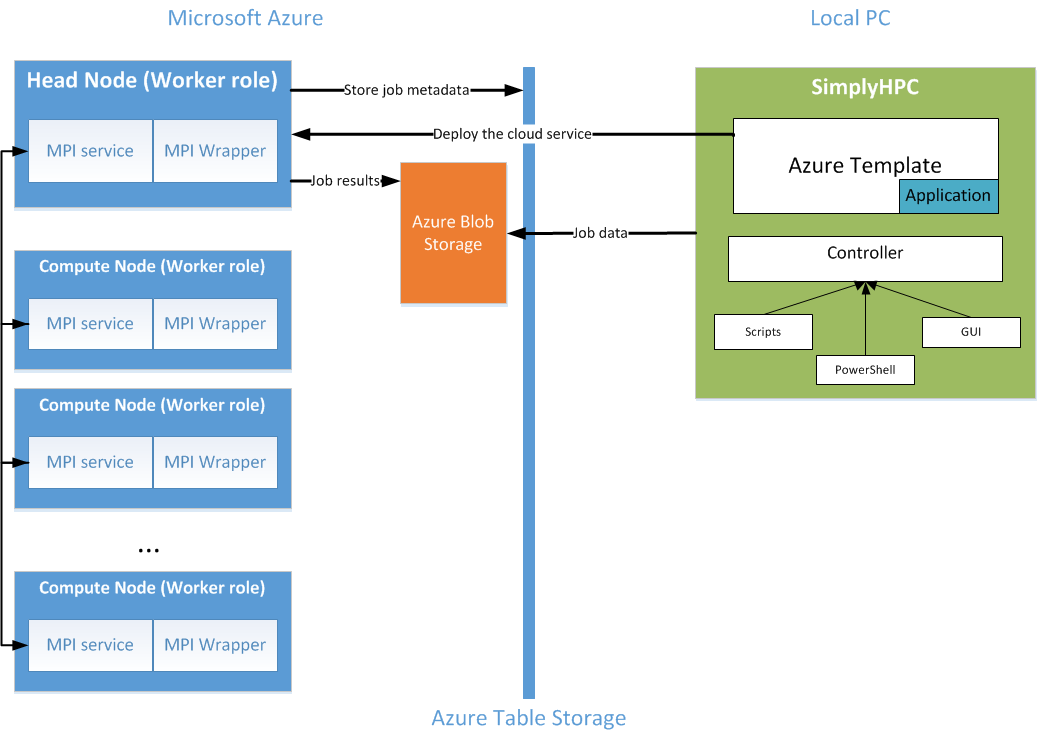
\includegraphics[width=10cm,height=7cm]{architecture.png}%
  \caption{Architecture of the SimplyHPC framework with the relationship between the modules and local and cloud resources.}
	\label{fig:architecture}
\end{figure}

% discuss the architecture

\subsection{Deployment procedure}
\label{sec:deploymentProcedure}

Deployment procedure is logically consistent with the natural way of running a job in the cluster and can be invoked entirely with the commandlets listed in Tab.~\ref{tab:CommandletsOfSimplyHPC}. During the procedure a cluster with the arbitrary number of VMs is created including the head and compute nodes, the job data get submitted to the Blob Storage, executed and after it finishes the results are retrieved and the cluster is destroyed while leaving the job results in the storage for later analysis. This includes the resulting data files, standard output and standard error. The whole process can be described as follows:
	
\begin{enumerate}

	\item \textit{NewAzureService} script creates the {\it Cloud Service} and configuration data like regional settings, logging and storage information are specified in a configuration file and stored in a separated variable (NewAzureParameters script). The application is not executed yet.

	\item \textit{NewAzureJob} script uploads the DTM to the Cloud Service. This script also effectively advises the Azure cloud to create the head and compute nodes as non-persistent virtual machines with a pre-installed and pre-configured operating system. They can be removed and recreated with the DTM template any time.  The CM controller then applies the deployment template to each of this machine and Microsoft MPI as well as a custom written job scheduler is installed. After this step, billing for the instances starts and the cluster is ready to be used.

	\item Jobs are uploaded to the Blob storage from a client computer. A job includes the executable and library files, data files and information about execution parameters, etc. The job is distributed to all the nodes automatically. 

	\item Using MPI, the head node executes the job on all nodes in the deployed cluster.

 	\item \textit{GetJobResults} script informs the node with the lowest id to upload the job results directly to the Azure Blob storage. Job results include log files, standard error/output of the process and any files that were newly created or changed by the running application.

	\item After running one or multiple jobs, the deployment can be removed with the \textit{RemoveAzureJobs}. This effectively stops billing as the virtual machines are deleted. Configuration data and reserved addresses are preserved.

	\item If no further deployments are needed, the cloud service is removed with the \textit{RemoveAzureService}. The job results remain intact in the Azure storage.

The only manual step in this case is to run \textit{NewAzureParameters} script to create a variable with configuration data. This variable is used by other remaining scripts. It is also assumed that Affinity Group and the Storage account have been created. This can be done very easily in the Azure Management Portal.

\end{enumerate}

%\begin{wrapfigure}{r}{0.2\textwidth}
               %
%\begin{tikzpicture}[shorten >=1pt,node distance=2.5cm,on grid,auto,anchor=east,scale=0.6, every node/.style={transform shape}] 
%
%\usetikzlibrary{shapes,arrows,positioning}
%\usetikzlibrary{decorations.pathreplacing, automata}
%
%\tikzstyle{every state}=[minimum size=18mm]
%
   %\node[state, align=center] (create)                     {1\\Create\\Service}; 
   %\node[state, align=center, below =of create] (deploy)   {2\\Deploy\\Template};    
   %\node[state, align=center, below= of deploy] (upload)   {3\\Upload\\Job}; 
   %\node[state, align=center, below =of upload] (run)      {4\\Run\\Job}; 
   %\node[state, align=center, below =of run] (retrieve)    {5\\Retrieve\\Results}; 
   %\node[state, align=center, below =of retrieve] (delete) {6\\Delete\\Dep.};
   %\node[state, align=center, below =of delete](delservice){7\\Delete\\Service};
   %
   %\path[->] 
   	%(create) edge  node {} (deploy)
   	%(deploy) edge  node {} (upload)
   	%(upload) edge   node {} (run)
   	%(run) edge   node {} (retrieve)
   	%(retrieve) edge [bend right=50 ]  node {} (upload)
   	%(retrieve) edge  node {} (delete)
   	%(delete) edge  node {} (delservice);
            %
  %\draw [decorate,decoration={brace,amplitude=20pt}]
 %(delete.west) -- (deploy.west) node [black,align=right,rotate=90,yshift=1cm,midway, xshift=1.5cm] { Billable Period};
  %\end{tikzpicture}
%
%\caption{Deployment process.}
%\label{fig:process}
 %\end{wrapfigure}

\begin{figure}
\centering
\begin{subfigure}{.5\textwidth}
  \centering
			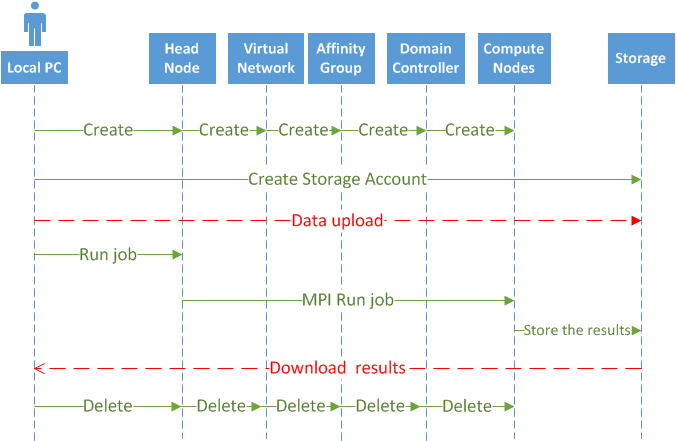
\includegraphics[width=\linewidth]{hpcPackSeq}	
  %\caption{A subfigure}
  \label{fig:hpcg}
\end{subfigure}%
\begin{subfigure}{.5\textwidth}
  \centering
  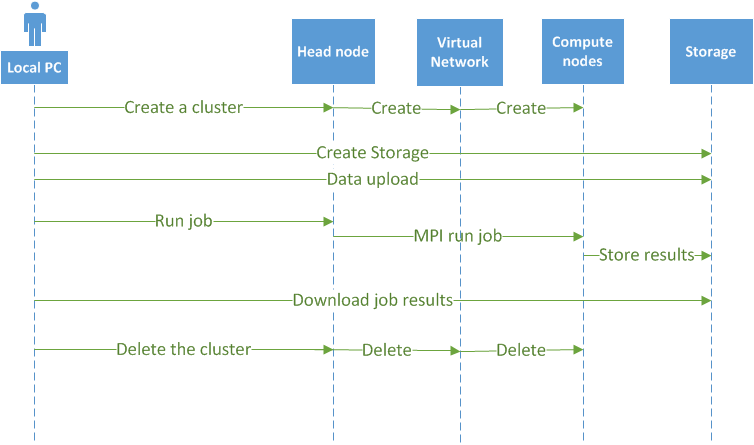
\includegraphics[width=\linewidth]{simplyHpcSeq}
  %\caption{A subfigure}
  \label{fig:cost}
\end{subfigure}
\caption{Sequential diagram of HPC Pack (left) and SimplyHPC framework (right). Dottet and solid lines refer to manual and automated processes, respectively.}
\label{fig:seqDiagram}
\end{figure}


There are manifold differences between SimplyHPC framework and HPC Pack. Although the HPC pack includes more features, such as scheduler or graphical user interface for job management, deployment with a HPC pack has certain disadvantages. First, the user needs a certain degree of expertise to be able to run HPC Pack as well as manual interaction with the head node which prohibits the automation. In contrary in SimplyHPC deployment procedure can be performed from the command line with a few configuration steps. Second, deploying a HPC Pack cluster needs a big infrastructure. For the simplest deployment it is required to have an MS SQL Database, Domain controller, a head node machine and every compute node being configured as a worker role. Such an infrastructure is usually not needed in case of scientific applications run from the command line. In our framework these entities have been removed from the procedure, therefore the head node can also take the role of the compute node, reducing the resources. \\
Third, creation time of a cluster with HPC Pack is much longer (see Fig.~\ref{fig:deployTime}). Fourth, HPC Pack does not provide a way to automatically check if the job has been successfully executed. If the user wants to reduce the costs and shut down the cluster once his jobs are finished he is forced to perform a manual check of the job status. In contrary, SimplyHPC framework allows to deploy a cluster, run jobs and delete the cluster automatically as soon as the jobs finished. %The windows service checks for the results in the job directory and results are uploaded to the storage. \\
Fifth, HPC Pack uses Microsoft MPI implementation that requires a Simple Multipurpose Daemon Service (SMPD) to run on every compute nodes. The installation of SMPD as a windows service is permitted to HPC Pack only which is a strong limitation is situation when the user wants to use another application to start and stop windows services. The proposed framework removes the limitation by creating a separated MPI service that automatically runs SMPD on every deployed virtual machine. \\
Last but least, after the initial deployment the user needs to move the job data to the Storage account manually and run the job from the HPC Pack Scheduler via Remote Desktop Connection or web interface. In SimplyHPC for command-line applications these tasks are performed automatically without user interaction (see Fig.~\ref{fig:seqDiagram}).
 

\section{Results}
\label{sec:results}
	
The tests were performed in Microsoft Azure cloud from the same subscription as well as in the private cluster. HSR Cluster is a privately owned and maintained cluster at Microsoft Innovation Center at University of Applied Sciences at Rapperswil (HSR), Switzerland. It is composed of $32$ nodes with 48GB RAM and two Intel Xeon E5645 6 cores each, the nodes are connected with 40Gbit Infiniband Network. On each Windows Server $2012$ R2 with HPC Pack 2012 R2. Microsoft provides description of the A8 and A9 nodes only. During the tests we used a cluster with multiple A8 and ExtraLarge instances.

\begin{figure}
\centering
\begin{subfigure}{.5\textwidth}
  \centering
	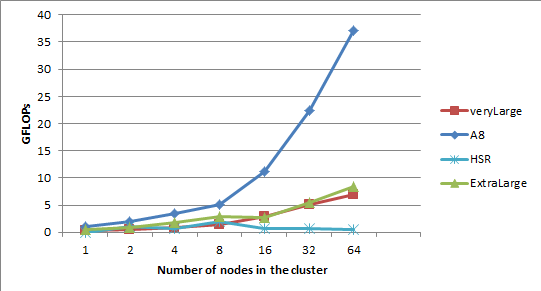
\includegraphics[width=\linewidth]{ruppel}  
  %\caption{A subfigure}
  \label{fig:ruepel}
\end{subfigure}%
\begin{subfigure}{.5\textwidth}
  \centering
  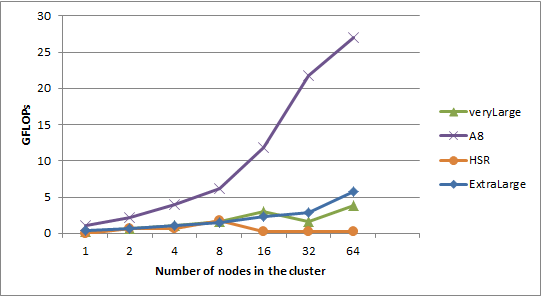
\includegraphics[width=\linewidth]{nord.png}
  %\caption{A subfigure}
  \label{fig:nord}
\end{subfigure}
\caption{Performance in GFlops of PETSc solving ruep (left) and nord (right) matrix systems on different Microsoft Azure nodes and a private HSR cluster. }
\label{fig:test}
\end{figure}
 
First objective was to compare deployment time of a cluster with different number of nodes in both systems. This time should be of the same order regardless the type of role instances because the deployment processes are similar, therefore we performed the tests with a one type of the role instances, namely A4 (see Tab.\ref{tab:azureVMs}). HPC Pack provides a precise statistics on the deployment procedure seperated into individual processes, namely creating a storage account, a virtual network, a cloud service, a domain controller as well as  deployment and configuration time for the head node and compute nodes. Since in SimplyAzure most of these processes were omitted, only the time to deploy the head node and compute nodes was measured, e.g. the time needed to run NewAzureService and NewAzureJob scripts (\textcolor[rgb]{1,0,0}{Vladimir, I noticed there is only one entry in the xls file}). Since HPC Pack neither provides automatic job submission nor does it retrieve the result we have not taken these processes into account in our measurements. 

%we measured the time needed create a cluster was measured together with other tasks, i.e. a time needed to pack and send the job to the cluster before the job starts executing.  

\begin{figure}
\centering
\begin{subfigure}{.5\textwidth}
  \centering
			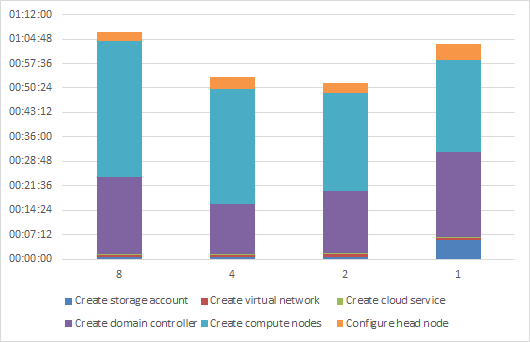
\includegraphics[width=\linewidth]{hpcDeployTime}	
  %\caption{A subfigure}
  \label{fig:hpcgDeploy}
\end{subfigure}%
\begin{subfigure}{.5\textwidth}
  \centering
  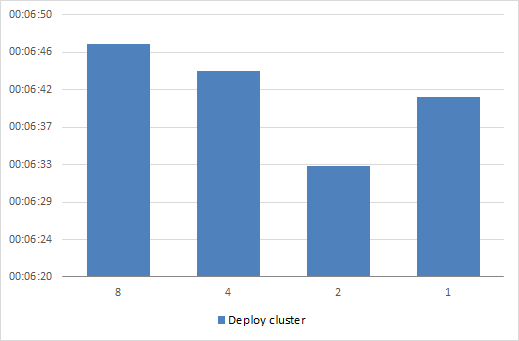
\includegraphics[width=\linewidth]{simplyHpcDeployTime}
  %\caption{A subfigure}
  \label{fig:simplyHpcDeploy}
\end{subfigure}
\caption{Deployment time of cluster composed of different number of A4 nodes with Microsoft HPC pack (left) and SimplyHPC framework (right). Time is provided in hh:mm:ss format.}
\label{fig:deployTime}
\end{figure}

Fig.~\label{fig:deployTime} shows the HPC Pack needs almost an hour to deploy the cluster while the SimplyHPC platform needs about six minutes in average. Such long deployment time lies in the fact HPC Pack performs also unnecessary deployment steps such as creating a domain controller or installing many additional services that are not needed for third-party scientific applications such as ZZZ (\textcolor[rgb]{1,0,0}{Vladimir, do you know why it takes that long?}).

The objective of the second experiment was to compare the performance of Microsoft Azure with a private cluster by running sparse matrix solver called PETSc. PETSc was run with two matrices: ruep and nord. The first one comes from thermal transient heat conduction simulation of electrical cabinet on a large unstructured mesh composed of 2.3 millions cells and the second matrix was generated from a thermal transient heat conduction simulation on a 3-dimensional Cartesian mesh of moderate size. Due to different mesh types, the second matrix converges much quicker than the first one. 

%Second, we compare the performance of a two framework by calculating how many typical PETSc simulations can be run on Microsoft Azure and in the local cluster in the same amount of time.


\begin{figure}
\centering
\begin{subfigure}{.5\textwidth}
  \centering
			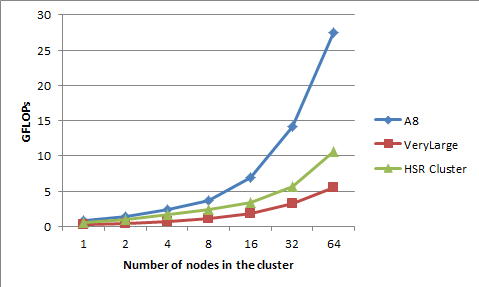
\includegraphics[width=\linewidth]{hpcg}	
  %\caption{A subfigure}
  \label{fig:hpcg}
\end{subfigure}%
\begin{subfigure}{.5\textwidth}
  \centering
  \includegraphics[width=\linewidth]{cost}
  %\caption{A subfigure}
  \label{fig:cost}
\end{subfigure}
\caption{Performance in GFlops of HPCG benchmark (left) and cost of a GFLOP in U.S. Dollars (right) on different Microsoft Azure nodes and a private HSR cluster. }
%\label{fig:cost}
\end{figure}

Since iterative solvers are memory-bound algorithms we measured the performance achieved for different combinations of cores in a single node, e.g. one node with one, two, four and eight cores and for two, four and eight nodes with eight cores. This way both vertical scaling (adding more cores to the system) and horizontal scaling (adding more nodes to the system) could be approximately measured. %More exact measurements were not executed because the private clusters had different hardware, the objective of the paper is different

HPCG benchmark test confirms the performance achieved on Azure nodes, although a slightly better performance was achieved for the HSR cluster due to suboptimal choice of the number of cores per node.  To illustrate this we run PETSc on HSR cluster with two, four and eight nodes with a single core. For ruep matrix the performance achieved was $2.1$, $4.1$ and $8.1$ GFLOPs, respectively. HPCG benchmark aims at solving a large sparse system of equation derived from a single degree of freedom heat diffusion model with zero Dirichlet boundary conditions. The global domain dimensions were $(nx * npx ) * (ny * npy ) * (nxz * npz )$ where $(nx * ny * nz )$ are the local subgrid dimension in the $x$, $y$, and $z$ dimensions, respectively, assigned to each MPI process. For the study $nx = ny = nz = 240$ and $npx, npy, npz$ are a factoring of the MPI process space that is computed automatically in the HPCG setup phase.


\subsection{Cost efficiency}

According to the IDC \cite{Perry2007} hardware generates only 7\% of Total Cost of Ownership (TCO) of a cluster operating for three years. Remaining costs are related to staffing, equipment, maintenance, middleware, and training. A yearly cost of a core hour $C_{core/h}$ can be calculated as follows \cite{ubercloud}:
$$ 
C_{core/h} = { C_p * T } / { N * 365 * 24 * U } 
$$
where $C_p$ is a cost of the cluster, $T$ is a TCO over a year being equal to $7\% * 1/3$ of the cluster cost, $N$ corresponds to the number of cores and $U$ is the average yearly utilization of the cluster. According to this formula $C_{core/h}$ is equal to $0.7\$$ with the average utilization of $30\%$. The price of the HSR cluster was $150k\$$ and according to the above equation, $C_{core/h}$ is $0.71$ for $100\%$ utilization of the system. Since the average utilization of HPC clusters is always much less. e.g. between $20$ and $30 \%$ \cite{Delimitrou:2014:QRQ:2541940.2541941} the price raises in more realistic scenarios (see Tab.~\ref{tab:cost}).

\begin{table}[h]
\begin{tabular}{lccccccccc}
\hline
\multicolumn{1}{|l|}{No. of nodes}          & \multicolumn{1}{c|}{1}       & \multicolumn{1}{c|}{2}      & \multicolumn{1}{c|}{3}     & \multicolumn{1}{c|}{8}    & \multicolumn{1}{c|}{10}     & \multicolumn{1}{c|}{12}    & \multicolumn{1}{c|}{16}   & \multicolumn{1}{c|}{24}   & \multicolumn{1}{c|}{32}   \\ \hline
\multicolumn{1}{|l|}{Utilization {[}\%{]}}  & \multicolumn{1}{c|}{0.03125} & \multicolumn{1}{c|}{0.0625} & \multicolumn{1}{c|}{0.125} & \multicolumn{1}{c|}{0.25} & \multicolumn{1}{c|}{0.3125} & \multicolumn{1}{c|}{0.375} & \multicolumn{1}{c|}{0.5}  & \multicolumn{1}{c|}{0.75} & \multicolumn{1}{c|}{100}  \\ \hline
\multicolumn{1}{|l|}{$C_{core/h}$ {[}\${]}} & \multicolumn{1}{c|}{22.65}   & \multicolumn{1}{c|}{11.32}  & \multicolumn{1}{c|}{5.66}  & \multicolumn{1}{c|}{2.83} & \multicolumn{1}{c|}{2.26}   & \multicolumn{1}{c|}{1.89}  & \multicolumn{1}{c|}{1.42} & \multicolumn{1}{c|}{0.94} & \multicolumn{1}{c|}{0.71} \\ \hline
                                            & \multicolumn{1}{l}{}         & \multicolumn{1}{l}{}        & \multicolumn{1}{l}{}       & \multicolumn{1}{l}{}      & \multicolumn{1}{l}{}        & \multicolumn{1}{l}{}       & \multicolumn{1}{l}{}      & \multicolumn{1}{l}{}      & \multicolumn{1}{l}{}     
\end{tabular}
\label{tab:cost}
\caption{Cost of the core per hour for different utilizations of the cluster. }
\end{table}

These calculations as well the price list in Tab.~\ref{tab:azureVMs} served to compare the cost of a single GFLOP in both systems. This metric was chosen to demonstrate the savings the cloud can bring in terms of performance since this is an important indicator when running numerical simulations (see Fig.\ref{fig:cost}). It turns out that even for less realistic utilization of the private cluster the cost for running in the cloud can be still lower in terms of computing power. For most realistic utilization of $30\%$ When the costs of a single GFLOP are compared directly it turns out the cloud can be much cheaper, especially for large deployment, for example running eight A8 machines can be 19 times cheaper as on the cluster. Therefore for small organizations a cloud may be an attractive alternative because it eliminates an up-front commitment and provides per-per-use option. SMEs can start small and only scale out when there is a need. The software is available at GitHub at https://github.com/vbaros/SimplyHPC.
 
% \todo[inline]{real life simulation, how much speed up, what's the effective use}

%\section{Related work}


\section{Conclusion}
\label{sec:conclusions}

We presented SimplyHPC framework, a novel distributed framework for Microsoft Azure Cloud. The framework is composed of light weight modules and a set of commandlets on top of that. The modules automate the complex deployment procedure that is necessary to run third-party applications from the local machine. In contrary to HPC Pack from Microsoft, all unnecessary system components and services have been omitted. As a result the time needed to deploy the cluster has been reduced from nearly an hour to couple of minutes.  This way scientific applications can access the cloud if the calculations are too time-consuming for a local machine or a private cluster. Specially designed mechanism keeps track of running jobs in the cluster. A special service in the head node regularly checks the job status and uploads the results to the blob storage as soon as the job finished successfully. Since a table and blob storage are distributed and mirrored, a high-availability and persistence of the job data is also provided.


%Further areas of work could include the following:

\section{Acknowledgments}
\label{sec:ackn}

The framework has been developed in Microsoft Innovation Center in Rapperswil, Switzerland and has been partly sponsored by Microsoft. 

\section{Literature}
\label{sec:literature}

\bibliography{hpconAzure}
\bibliographystyle{plain}

\end{document}

